\documentclass[a4paper]{ifacconf}

\usepackage[utf8]{inputenc}
\usepackage[T1]{fontenc}
\usepackage[english]{babel}
\usepackage{graphicx}
\usepackage{amsmath}
\usepackage{url} 
\usepackage[round]{natbib}             

% Added packages
\usepackage[dvipsnames]{xcolor}
\usepackage{tikz}
    % Useful libs (TiKz and Dvipsnames packages are assumed loaded)
\usetikzlibrary{
    shapes, 
    positioning, 
    decorations.pathmorphing, 
    decorations.markings,
    patterns,
    calc,
}

% Colors
\definecolor{startstop}{HTML}{FF3867}
\definecolor{io}{HTML}{2E8B57}
\definecolor{process}{HTML}{1CA1DA}
\definecolor{decision}{HTML}{D8C303}

% Spring and damper
\tikzstyle{spring}=[
    decorate, 
    decoration={
        coil,
        segment length = 1mm,
        amplitude = 1mm,
    }
]
\tikzstyle{damper}=[
    decoration={
    markings,  
      mark connection node=dmp,
      mark=at position 0.5 with 
      {
        \node (dmp) [thick,inner sep=0pt,transform shape,rotate=-90,minimum width=5pt,minimum height=1pt,draw=none] {};
        \draw [thick] ($(dmp.north east)+(1pt,0)$) -- (dmp.south east) -- (dmp.south west) -- ($(dmp.north west)+(1pt,0)$);
        \draw [thick] ($(dmp.north)+(0,-3pt)$) -- ($(dmp.north)+(0,2pt)$);
      }
    }, 
    decorate
]

% Flowchart blocks
\tikzstyle{startstop} = [
    rectangle, 
    rounded corners, 
    minimum width=2cm, 
    minimum height=1cm,
    text centered, 
    draw=black, 
    fill=startstop!50,
]

\tikzstyle{process} = [
    rectangle, 
    minimum width=2cm, 
    minimum height=1cm, 
    text centered, 
    draw=black, 
    trapezium stretches=true,
    fill=process!50,
]
\tikzstyle{io} = [
    trapezium, 
    trapezium left angle=70, 
    trapezium right angle=110, 
    minimum width=2cm, 
    minimum height=1cm, 
    text centered, 
    draw=black, 
    trapezium stretches=true,
    fill=io!30,
]
\tikzstyle{decision} = [
    diamond, 
    minimum width=1cm, 
    minimum height=1cm, 
    text centered, 
    draw=black, 
    fill=decision!50,
]

% Control diagram blocks
\tikzstyle{sum} = [
    draw,
    circle,
    minimum size=0.6cm,
    fill=Rhodamine!70,
]
% When using a sum shape, lines must be drawn and +- sign indicated
% \draw 
% (sum.north east) -- (sum.south west)
% (sum.north west) -- (sum.south east);
% \node[left=-1pt] at (sum.center){\tiny $+$};
% \node[below] at (sum.center){\tiny $-$};
\tikzstyle{controller} = [
    draw,
    fill=Peach!90,
    minimum width=1.2cm,
    minimum height=0.9cm,
]
\tikzstyle{system} = [
    draw,
    fill=Peach!90,
    minimum width=1.2cm,
    minimum height=0.9cm,
]
\tikzstyle{sensor} = [
    draw,
    fill=Goldenrod!80,
    minimum width=1.2cm,
    minimum height=0.9cm,
]
\usepackage{bm}
\usepackage{multicol}
\usepackage{multirow}
\usepackage{subcaption}
\usepackage{amssymb}
% ---

% Added commands
\definecolor{reviewcolor}{HTML}{fb3257}
\newcommand{\reviewmode}{0}
\newcommand{\reviewchange}[2]{%
    \if\reviewmode1%
        \color{reviewcolor}
            #2
        \color{black}
    \else%
        #2
    \fi   
}
% ---

\begin{document}


\begin{frontmatter}
    \title{%
        Error-Based Active Disturbance Rejection Control for Parkinson's Disease Tremor Suppression in Wrist Considering Upper Limb Dynamics\thanksref{footnoteinfo}
    }  
    
    \thanks[footnoteinfo]{%
        Financiamento: em parte pela FAPDF no. 435/2023 Processo nº~00193-00002143/2023-02, CHAMADA PÚBLICA 01/2023 BIO LEARNING / VINCULADA AO EDITAL 10/2023 - PROGRAMA FAPDF LEARNING Programa de Fomento Estratégico na macro área da linha de pesquisa: BIO Learning; em parte pelo Programa de Formação de Recursos Humanos da Agência Nacional do Petróleo, Gás Natural e Biocombustíveis.
    }
    
    \author[First]{Thiago T. de Paula} 
    \author[Second]{Matheus T. de Sousa} 
    \author[Second]{Jos\'e Oniram de A. Limaverde Filho}
    \author[First]{Marcela R. Machado}
    
    \address[First]{%
        Department of Mechanical Engineering, University of Brasília, DF 
        (e-mails: thiagotomasdepaula@gmail.com; marcelam@unb.br).
    }
    \address[Second]{%
        Department of Electrical Engineering, University of Brasília, DF 
        (e-mails: matheus.sousa@ieee.org; jose.oniram@ene.unb.br).
    }
       
    \renewcommand{\abstractname}{{\bf Abstract:~}}   

    \begin{abstract} % Abstract of not more than 250 words.
        Parkinson's disease is a neurodegenerative disorder whose tremor often persists despite pharmacological or surgical treatment. Active orthoses are a noninvasive alternative for wrist tremor suppression, but most approaches focus on single-joint compensation and neglect dynamic coupling from proximal joints. This work proposes an error-based active disturbance rejection control strategy for wrist tremor suppression using a three-degree-of-freedom upper limb model. The controller estimates and rejects total disturbances in real time, including model uncertainties and perturbations originating from proximal joints. Voluntary motion is estimated via \reviewchange{}{lowpass} filtering, and the method is evaluated against \reviewchange{}{proportional integral derivative} controllers. Simulation results over 100 trials for two different motion profiles show that 
        the method achieves a balance between tremor reduction and control effort. Although an optimized proportional integral derivative controller achieves higher suppression under ideal conditions, it requires prior knowledge of voluntary motion and higher actuation. In contrast, the method maintains significant attenuation and robustness to parameter variations, indicating its potential for practical wearable tremor suppression systems.
    \end{abstract}

    \begin{keyword}
        % Five to ten keywords, preferably chosen from the IFAC keyword list.
        Parkinson's Disease,
        Tremor Suppression,
        Voluntary Motion Tracking,
        Human-Machine Systems,
        Active Disturbance Rejection Control,
        Upper Limb Modeling.
    \end{keyword}

\end{frontmatter}

\section{Introduction}

\reviewchange{Parkinson's disease (PD) is a chronic, progressive neurodegenerative disorder primarily characterized by the substantial loss of dopaminergic neurons in the substantia nigra
\citep{Nguyen:2021, Fujikawa:2023, Meng:2022}.
This neurological decline results in a set of cardinal motor manifestations, including bradykinesia (slowness of movement), rigidity (stiffness), postural instability, and a characteristic unilateral rest tremor
\citep{Nguyen:2021, Botzel:2014}. 

Pharmacological therapy remains the first-line approach for tremor management, primarily relying on dopamine replacement through Levodopa or dopamine agonists \citep{Botzel:2014, Lora-Millan:2021}. However, long-term pharmacotherapy often leads to reduced effectiveness and may induce side effects including dyskinesia and motor fluctuations \citep{Lora-Millan:2021, Meng:2022}. In addition, a significant portion of patients does not respond adequately to medication \citep{Fujikawa:2023}. Surgical interventions such as Deep Brain Stimulation are considered in severe or refractory cases \citep{Botzel:2014, Fujikawa:2023}, although their invasive nature and associated risks limit their applicability. Complementary strategies, including occupational therapy and assistive tools, are also adopted to mitigate functional impairment \citep{Mo:2021, Bhidayasiri:2022}.

Orthotic devices are a less invasive alternative and can be classified as passive or active. Passive orthoses rely on mechanical elements or smart materials to attenuate tremor by dissipating vibratory energy at specific frequencies \citep{Gebai:2018, Moura:2025}, but are sensitive to variations in tremor frequency and require further validation in real-world conditions \citep{Heide:2014, Bhidayasiri:2022}. Active orthoses, in contrast, employ closed-loop control strategies that estimate tremor characteristics in real time and apply compensatory actions through mechanical loading or electrical stimulation \citep{Lora-Millan:2021, Meng:2022}.

Active control approaches introduce additional challenges due to their reliance on sensing, actuation, and real-time computation, which may reduce user comfort and cause fatigue \citep{Lora-Millan:2021, Martinez-Nunez:2024}. In particular, peripheral or functional electrical stimulation techniques may also induce discomfort and skin irritation or fatigue \citep{Taheri:2015, Saleh:2022}. Despite this, advances in hardware miniaturization and signal processing ensure their relevance, especially in wrist tremor suppression.

Several control strategies for wrist tremor suppression have been proposed in the literature. \cite{Gallego:2013} design a neuroprosthesis based on Proportional Integrative (PI) control for a single degree of freedom (DoF) system of the human wrist, combining a Critically Damped g-h Filter (CDF), a Weighted Frequency Fourier Linear Combiner (WFLC), and a Kalman filter for tremor estimation. \cite{Copur:2019} propose a zero-phase high-pass filter for tremor estimation alongside a repetitive control strategy for electrical stimulation-based co-contraction in a single DoF setup.

In parallel, \cite{Lekshmi:2019} introduce a Proportional Integrative Derivative (PID) controller applied to a four DoF wrist model with gains optimized via genetic algorithm. \cite{Zamanian:2019} develop an adaptive notch filter supported by an Adaptive Frequency Estimator (AFE) to track tremor frequency in the velocity signal. More recently, \cite{Qi:2024} propose an Active Disturbance Rejection Control (ADRC) strategy using an Enhanced Bandlimited Multiple Fourier Linear Combiner (EBMFLC) for voluntary motion estimation.

Most approaches focus on single-joint models, where excellent results have been achieved, but do not account for dynamic coupling between joints, where shoulder and elbow PD tremors significantly affect wrist motion. To address this issue, a 3-DoF linear upper limb model proposed in \citep{Gebai:2017, Gebai:2018} is adopted in this work as a test platform.

In this scenario, disturbance rejection-based control methods are expected to offer advantages due to their robustness to model uncertainties and external perturbations. This work investigates an error-based active disturbance rejection control for wrist tremor suppression under coupled dynamics. Two variations are considered, differing in how voluntary motion is estimated: one based on EBMFLC (following after \cite{Qi:2024}) and another on Zero-Phase Low-Pass (ZPLP) filtering. 
These are compared against AFE,  
the PI proposed by \cite{Gallego:2013}, and two PID controllers, one tuned with Internal Model Control (IMC) and the other with offline Differential Evolution (DE) optimization. 
Robustness is evaluated through Monte Carlo simulations of physical parameters.

The remainder of this paper is organized as follows: Section \ref{sec:theory} presents the upper limb dynamic model and the control framework. Section \ref{sec:methodology} describes the simulation setup. Section \ref{sec:results} discusses the obtained results. Section \ref{sec:conclusion} concludes the paper and outlines future work.}{
Parkinson's disease (PD) is a chronic, progressive neurodegenerative disorder primarily characterized by the substantial loss of dopaminergic neurons in the substantia nigra
\citep{Meng:2022,Fujikawa:2023}.
This neurological decline results in a set of cardinal motor manifestations, including bradykinesia (slowness of movement), rigidity (stiffness), postural instability, and a characteristic unilateral rest tremor
\citep{Botzel:2014}. 

Pharmacological therapy 
\citep{Botzel:2014, Lora-Millan:2021}
remains the first-line approach for tremor management, 
but a significant portion of patients does not respond adequately to medication \citep{Fujikawa:2023},
and long-term pharmacotherapy often leads to reduced effectiveness and may induce debilitating side effects \citep{Lora-Millan:2021, Meng:2022}. 
Surgical interventions \citep{Botzel:2014, Fujikawa:2023} may be considered, but invasiveness and risks limit their applicability. 

Actively controlled orthoses are an effective, non-invasive alternative 
\citep{Lora-Millan:2021, Meng:2022}, 
and particularly popular for wrist tremor suppression.

Several control strategies for wrist tremor suppression have been proposed in the literature. \cite{Gallego:2013} design a neuroprosthesis based on Proportional Integrative (PI) control for a single degree of freedom (DoF) system of the human wrist, combining a Critically Damped g-h Filter (CDF), a Weighted Frequency Fourier Linear Combiner (WFLC), and a Kalman filter for tremor estimation. \cite{Copur:2019} propose a zero-phase high-pass filter for tremor estimation alongside a repetitive control strategy for electrical stimulation-based co-contraction in a single DoF setup.

In parallel, \cite{Lekshmi:2019} introduce a Proportional Integrative Derivative (PID) controller applied to a four DoF wrist model with gains optimized via a genetic algorithm. \cite{Zamanian:2019} develop an adaptive notch filter supported by an Adaptive Frequency Estimator (AFE) to track tremor frequency in the velocity signal. 
More recently, \cite{Qi:2024} propose an Active Disturbance Rejection Control (ADRC) strategy using an Enhanced Bandlimited Multiple Fourier Linear Combiner (EBMFLC) for voluntary motion estimation.

While shoulder and elbow PD tremors significantly affect wrist motion,
most approaches focus on single-joint models, neglecting joint coupling. 
To address this issue, a 3-DoF linear upper limb model 
\citep{Gebai:2017, Gebai:2018} 
is adopted in this work as a test platform.

Disturbance rejection-based control 
\citep{Guo:2016}
is expected to offer advantages due to its robustness to external perturbations and model uncertainties. 
This work investigates an error-based active disturbance rejection control for wrist tremor suppression under coupled dynamics. Two variations are considered, differing in how voluntary motion is estimated: one based on EBMFLC \cite{Qi:2024} and another on Zero-Phase Low-Pass (ZPLP) filtering. 
These approaches are evaluated against two PID controllers, one tuned with Internal Model Control (IMC) and the other with offline Differential Evolution (DE) optimization plus perfect knowledge of voluntary motion. 
Robustness is evaluated through Monte Carlo simulations of physical parameters.
}

The remainder of this paper is organized as follows: Section \ref{sec:theory} presents the upper limb dynamic model and the control framework. Section \ref{sec:methodology} describes the simulation setup. Section \ref{sec:results} discusses the obtained results. Section \ref{sec:conclusion} concludes the paper and outlines future work.

\section{Theoretical Framework}
\label{sec:theory}

    \subsection{Upper Limb Model}
    
    The upper limb is modeled as a planar three DoF system, where the shoulder, elbow, and wrist joints define the generalized coordinates. Following \cite{Gebai:2018}, muscles and tendons are represented as equivalent springs and dampers, resulting in the schematic shown in Figure \ref{fig:system}. The system dynamics are described by
    \begin{equation}
        \mathbf{J}\ddot{\bm{\theta}} +
        \mathbf{C}\dot{\bm{\theta}} +
        \mathbf{K}\bm{\theta}
        =
        \bm{\tau},
    \label{eq:system}
    \end{equation}
    
    \begin{figure}[htbp]
        \centering
        \caption{
            Human upper limb simplified mechanical representation. 
            Adapted from \cite{Albuquerque:2025}.
        }
        \label{fig:system}
        \begin{tikzpicture}[scale=1.066, > = latex]

    % Invisible vertical padding
    \draw [white] (0,2.75) circle (1);

    \node [opacity=0.25] at (0,0) {
        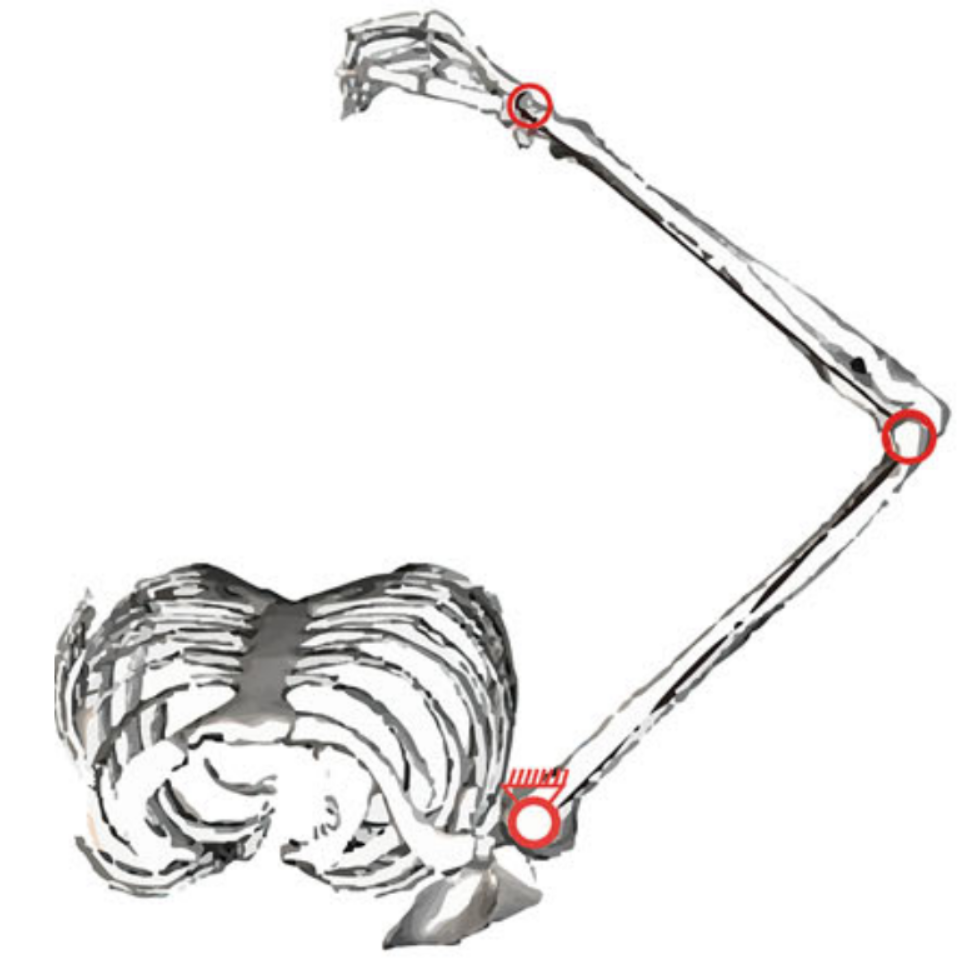
\includegraphics[width=0.8\linewidth]
        {figures/skeleton.png}
    };
    
    \coordinate (shoulder) at (0.37, -2.37);
    \path (shoulder) +(45.9:3.725) coordinate (elbow);
    \path (elbow) +(138.7:3.47) coordinate (wrist);
    \path (wrist) +(138.7:0.9) coordinate (knuckle);
    
    % test coordinates alignments (debug only)
    % \draw [cyan, fill=cyan, opacity=0.2, thick, dashed] (shoulder) circle (0.3);
    % \draw [cyan, fill=cyan, opacity=0.2, thick, dashed] (elbow) circle (0.3);
    % \draw [cyan, fill=cyan, opacity=0.2, thick, dashed] (wrist) circle (0.3);
    % \draw [cyan, fill=cyan, opacity=0.2, thick, dashed] (knuckle) circle (0.3);

    % Arm annotations
    \draw [|-|, opacity=0.5] (shoulder) ++ (-45:0.5) --++ (45.9:3.725)
        node [midway, fill=white, opacity=1.0, inner sep=0.2] {$l_1$};
    \draw [thick, orange, fill=orange, opacity=0.5]
        (shoulder) ++ (0.2, 0) 
        --++ (0.7, 0) node [right, black, opacity=1.0] {$\theta_1$}
        arc (0:45.9:0.7) -- cycle;
    \draw [thick, <->] (shoulder) ++ (0.5, 0) arc (0:90:0.5) 
        node [midway, above, xshift=0.4cm, yshift=-0.1cm] {$I_1, \tau_1$};

    % Forearm annotations
    \draw [|-|, opacity=0.5] (elbow) ++ (45:0.55) --++ (142:3.5)
        node [midway, fill=white, opacity=1.0, inner sep=0.2] {$l_2$};
    \draw [thick, orange, fill=orange, opacity=0.5]
        (elbow) ++ (42:0.35) 
        --++ (45:0.7) arc (45:142:0.7) 
        node [midway, above, black, opacity=1.0] {$\theta_2$}
        -- cycle;
    \draw [thick, <->] (elbow) ++ (175:0.3)
        arc (180:90:0.5) node [below, xshift=0.2cm, yshift=-0.2cm] {$I_2, \tau_2\quad$};

    % Wrist annotations
    \draw [|-|, opacity=0.5] (wrist) ++ (45:0.3) --++ (138:0.9)
        node [midway, fill=white, opacity=1.0, inner sep=0.2] {$l_3$};
    \draw [thick, orange, fill=orange, opacity=0.5]
        (wrist)
        --++ (142:0.7) 
        arc (142:135:0.7) 
        node [midway, left, black, opacity=1.0] {$\theta_3$} 
        -- cycle;
    \draw [thick, <->] (wrist) node [xshift=0.1cm, yshift=0cm] {$I_3, \tau_3$} ++ (100:0.3)
        arc (100:170:0.4) ;

    % Stiffness and damping
    
    %% Shoulder
    \draw [spring] (shoulder) ++ (97:1.05) arc (97:45:1.05);
    \draw [postaction={damper}] (shoulder) ++ (98:1.3) arc (98:45:1.3)
        node [midway, above, sloped, yshift=0.1cm] {$k_1$, $c_1$};
        
    %% Elbow            
    \draw [spring] (elbow) ++ (-135:0.5) arc (-135:-225:0.5);
    \draw [postaction={damper}] (elbow) ++ (-135:0.8) 
    arc (-135:-225:0.8)
    node [midway, above, sloped, yshift=0.1cm] {$k_2$, $c_2$};
    %% Biceps
    \draw [spring] (elbow) ++ (-135:3.7) arc (-135:-280:2);
    \draw [postaction={damper}] (elbow) ++ (-135:4) 
        arc (-135:-270:2.3)
        node [midway, above, sloped, yshift=0.1cm] {$k_3$, $c_3$};
    %% Wrist
    \draw [spring] (wrist) ++ (175:0.5) arc (175:317:0.5);
    \draw [postaction={damper}] (wrist) ++ (176:0.8) 
        arc (176:317:0.8)
        node [midway, below, sloped] {$k_4$, $c_4$}; 
    
\end{tikzpicture}
    \end{figure}
    
    where $\bm{\theta} = [\theta_1\ \theta_2\ \theta_3]^\top$ denotes the joint flexion angles at the shoulder, elbow, and wrist, respectively, and $\bm{\tau}$ is the vector of applied torques. 
    %
    \reviewchange{}{The linearized model is a fair representation of dynamics as long as physical parameters' change in time is small \citep[section 4.2.2]{Gebai:2020}.}
    %
    The inertia, stiffness, and damping matrices are given by
    \begin{equation}
    \begin{aligned}
        &\mathbf{J} =
        \begin{bmatrix}
            j_{11} & j_{12} & j_{13} \\
                   & j_{22} & j_{23} \\
            \text{sym.} & & j_{33}
        \end{bmatrix}, \quad 
        \mathbf{K} =
        \begin{bmatrix}
            k_1 + k_3 & k_3       & 0 \\
            k_3       & k_2 + k_3 & 0 \\
            0         & 0         & k_4
        \end{bmatrix},\\[1mm]
        &\mathbf{C} =
        \begin{bmatrix}
            c_1 + c_3 & c_3       & 0 \\
            c_3       & c_2 + c_3 & 0 \\
            0         & 0         & c_4
        \end{bmatrix}.
    % \label{eq:KC}
    \end{aligned}
    \end{equation}
    
    The upper limb is composed of three rigid segments representing the arm, forearm, and hand, with masses $m_1$, $m_2$, and $m_3$, lengths $l_1$, $l_2$, and $l_3$, and moments of inertia $I_1$, $I_2$, and $I_3$. The distances from each joint to the segment's center of mass are denoted by $a_1 = 0.427l_1$, $a_2 = 0.417l_2$, and $a_3 = 0.361l_3$
    \reviewchange{}{\citep{Gebai:2018}.}
    Joint stiffness is modeled through parameters $k_1$, $k_2$, and $k_4$, corresponding to the shoulder, elbow, and wrist, respectively, while $k_3$ represents the coupling stiffness associated with the biceps. Damping coefficients $c_i$ are assumed proportional to stiffness, such that $c_i \propto k_i$ for $i \in \{1,\ 2,\ 3,\ 4\}$.
    
    The inertia matrix elements are defined as
    \begin{align}
        j_{11} &= (I_1 + m_1 a_1^2) + m_2 l_1^2 + m_3 l_1^2 + j_{12}, \\
        j_{12} &= (I_2 + m_2 a_2^2) + m_3 (l_2^2 + l_2 a_3) + j_{13}, \\
        j_{13} &= m_3 (a_3^2 + l_2 a_3), \\
        j_{22} &= j_{12}, \quad
        j_{23} = j_{13}, \quad 
        j_{33} = I_3 + m_3 a_3^2.
    \end{align}
    
    Finally, tremor disturbances at each joint are characterized by amplitudes $A_i$ and frequencies $f_i$, for $i \in \{1, 2, 3\}$, corresponding to the shoulder, elbow, and wrist.

    For a patient with PD, $\bm{\tau}$ is part voluntary, part involuntary.
    Denoting the pathological torque by $\bm{\tau}_i$ and the voluntary torque by $\bm{\tau}_v$,
    equation \eqref{eq:tau} is written \citep{Qi:2024}:
    %
    \begin{equation}
        \bm{\tau} = \bm{\tau}_i + \bm{\tau}_v.
    \label{eq:tau}
    \end{equation}

    \reviewchange{where we've modeled $\bm\tau_i$ by \eqref{eq:tau_PD}:}{%
        Most of a PD tremor's power is narrowly concentrated around a central frequency
        \citep{Deuschl:2022}.
        Typically, tremor
        is approximated by up to 3 harmonics,
        whose frequencies the controller attempts to identify and reject
        \citep{Zamanian:2019,Albuquerque:2025}.
        Since joint coupling naturally makes wrist dynamics multimodal, 
        we've modeled $\bm\tau_i$ as 1 harmonic per joint:
    }
    \begin{equation}
        \bm{\tau}_i = 
        \begin{bmatrix} 
            A_1\sin(2\pi f_1 t) &
            A_2\sin(2\pi f_2 t) &
            A_3\sin(2\pi f_3 t) 
        \end{bmatrix}^\top.
    \label{eq:tau_PD}
    \end{equation}

    By defining the state vector as
    %
    $\mathbf{x} = 
    \begin{bmatrix} 
        \bm{\theta}^\top & 
        \dot{\bm{\theta}}^\top
    \end{bmatrix}^\top$,
    %
    the state space representation in 
    \eqref{eq:state_space_x} of the dynamic in \eqref{eq:system} is straightforwardly obtained:
    %
    \begin{align}
        \dot{\mathbf{x}} 
        &=
        \mathbf{A}\mathbf{x} + \mathbf{B}\bm{\tau} 
    \label{eq:state_space_x}
        \\
        \mathbf{y} 
        &= 
        \mathbf{C}_\text{ss}
        \mathbf{x} 
    \label{eq:state_space_y}
    \end{align}
    %
    \begin{equation*}
        \mathbf{A} =
        \begin{bmatrix}
            \mathbf{0} & \mathbf{I} \\
            -\mathbf{J}^{-1}\mathbf{K} & -\mathbf{J}^{-1}\mathbf{C}
        \end{bmatrix},
        \quad
        \mathbf{B} =
        \begin{bmatrix}
            \mathbf{0} \\
            \mathbf{J}^{-1}
        \end{bmatrix},
        \quad
        \mathbf{C}_\text{ss} = 
        \begin{bmatrix}
            \mathbf{I} &
            \mathbf{0}
        \end{bmatrix},
    % \label{eq:C_ss}
    \end{equation*}
    %
    where $\mathbf{0}$ and $\mathbf{I}$ are 3$\times$3 null and identity matrices.
    
    \subsection{Error-based ADRC}
    \label{sec:adrc}
    
    The ADRC is a control paradigm focused on real-time estimation and rejection of the total disturbance. This includes both internal model uncertainties and exogenous disturbances \citep{Guo:2016}. The classical formulation uses measurements of the plant output $y(t)$ to estimate system states and disturbances via an extended state observer. Consider a general $n$-th order Single-Input Single-Output (SISO) system:
    \reviewchange{%
        \begin{equation}
            y^{(n)}(t) = f(y, \dot{y}, \dots, y^{(n-1)}, w, t) + b_0 u(t),
        \label{eq:general_system}
        \end{equation}
    }{%
        \begin{equation}
            y^{(n)}(t) = f(y, \dot{y}, \dots, y^{(n-1)}, t) + b_0 u(t),
        \label{eq:general_system}
        \end{equation}
    }
    where $y(t)$ is the output, $u(t)$ the control input, $b_0$ the high-frequency gain, and $f(\cdot)$ the total disturbance.
    
    Error-based ADRC (EADRC) defines control in terms of the tracking error $e(t) = r(t) - y(t)$ instead of the plant output, which simplifies implementation and is well suited for practical applications \citep{Madonski:2019}. For the system in \eqref{eq:general_system}, the error dynamics are given by:
    \begin{equation}
        e^{(n)}(t) = r^{(n)}(t) - y^{(n)}(t) = r^{(n)}(t) - f(\cdot) - b_0 u(t).
    \end{equation}
    
    Defining $f_e(t) = r^{(n)}(t) - f(\cdot)$ yields
    \begin{equation}
        e^{(n)}(t) = f_e(t) - b_0 u(t),
    \label{eq:error_siso}
    \end{equation}
    which retains the canonical ADRC structure in the error domain. Then, by defining the extended state vector as:
    \begin{equation}
        z_1 = e,\quad z_2 = \dot{e},\quad \dots,\quad z_n = e^{(n-1)},\quad z_{n+1} = f_e,
    \end{equation}
    the corresponding error-based extended state observer can be written as:
    \begin{equation}
    \begin{cases}
        \dot{\hat{z}}_1 = \hat{z}_2 + \beta_1 (e - \hat{z}_1), \\
        \dot{\hat{z}}_2 = \hat{z}_3 + \beta_2 (e - \hat{z}_1), \\
        \vdots \\
        \dot{\hat{z}}_n = \hat{z}_{n+1} + \beta_n (e - \hat{z}_1) - b_0 u, \\
        \dot{\hat{z}}_{n+1} = \beta_{n+1} (e - \hat{z}_1).
    \end{cases}
    \label{eq:eeso_n}
    \end{equation}
    Control law is then defined as a regulator in the error coordinates:
    \begin{equation}
        u(t) = \frac{\sum_{i=1}^{n} \kappa_i \hat{z}_i(t) - \hat{z}_{n+1}(t)}{-b_0},
    \label{eq:control_law_error}
    \end{equation}
    where $\kappa_i$ are the controller gains chosen to achieve the desired closed-loop dynamics.

    \reviewchange{}{\subsubsection{Concerns}
        While ADRC converges quickly and its implementation is simple (specially EADRC's), unstability in the observer may cause computational problems.
        %
        \textit{Ad hoc} solutions such as control signal magnitude/rate limitation are often employed in this case \citep{Herbst:2025}.
    }

\section{Methodology}
\label{sec:methodology}

\subsection{Tracking error}
The observed value of wrist angle flexion $\theta_3$ is composed by two parts,
a voluntary portion due to voluntary torque from the patient, 
and an involuntary portion due to PD tremor, i.e.:
%
\begin{align}
    \theta_3 
    &= 
        \underbrace{\theta_{v_3}}_{\text{Due to } \tau_{v_3}} + 
        \underbrace{\theta_{i_3}}_{\text{Due to } \tau_{i_3}}
\end{align}
%
since the simplified system is linear.
%
We wish to dampen the tremor at the wrist by applying a torque $u_3$ to it.
With respect to the modeling, this means adding a vector 
$\mathbf{u} = 
\begin{bmatrix}
    0 & 0 & u_3
\end{bmatrix}^\top$
to $\bm{\tau}$.
%
Isolating the dynamics at the wrist ($\theta_3$) from the state-space representation in \eqref{eq:system}, the following is derived:
%
\begin{equation}
    \ddot{\theta}_3 
    = 
    b_0 u_3 +
    \zeta(\bm{\tau}, \bm{\theta}, \dot{\bm{\theta}}),
\label{eq:wrist_dynamic}
\end{equation}
% 
where $b_0$ is the $(3,3)$ entry of $\mathbf{J}^{-1}$, and $\zeta$ is a linear combination of $\bm{\theta}$, $\dot{\bm{\theta}}$, and $\bm{\tau}$.

Ideally, the ESO tracking error would be given by
%
\begin{equation}
    e_3(t) 
    = \theta_{i_3}(t)
    = \theta_{v_3}(t) - \theta_3(t),
\end{equation}

so that $e_3\to 0$ as $u_3$ compensates $\tau_{i_3}$.

In a practical setting, $\theta_{v_3}$ is unknown, 
and thus we estimate the tracking error using
%
\begin{equation}
    \widehat{e}_3(t) 
    = \widehat{\theta}_{v_3}(t) - \theta_3(t),
\label{eq:e3_hat}
\end{equation}
%
where $\widehat{\theta}_{v_3}$ is an estimate of $\theta_{v_3}$.
From \eqref{eq:e3_hat}, 
we have that $\widehat{e}_3 \to \epsilon_3$
as $u_3$ compensates $\tau_{i_3}$,
where $\epsilon_3$ is the voluntary motion estimator error.
    
    
\subsection{Simulation Setup}

Controller performance is evaluated through repeated simulations under varying physical conditions. For each run, upper limb parameters are sampled around nominal values as described in Subsection \ref{sec:parameters}, and the system response is simulated and evaluated. This procedure is repeated to assess robustness. Since involuntary torques due to Parkinson's disease are already modeled, only voluntary torque profiles are specified. Voluntary torques are null to emulate resting, and to emulate motion follow the trajectories described in Section \ref{sec:results}.

Performance is assessed using output-based and control-based metrics. 
For the wrist joint, Tremor Power Suppression Ratio (TPSR) \citep{Qi:2024}, 
Integral Absolute Error (IAE) \citep{Skogestad:2003}, 
Coefficient of Determination ($R^2$) \citep{Glantz:1990}, and 
Entropy \citep{Lathi:2018} are computed. 
Control effort is evaluated through the 
Total Variation (TV) \citep{Skogestad:2003} and 
Signal Power \citep{Lathi:2018} of the control input.

\subsection{Parameters}
\label{sec:parameters}

\subsubsection{Model Parameters}
% Nominal parameters and range from which they were sampled
Between system simulations, stiffness coefficients change according to samples drawn from uniform distributions centered at their nominal values, which also cause damping coefficients to change since they are associated to stiffness.
The very first run of each control strategy is run with the nominal model, and following runs use altered models for a total of 100 runs. 
The 99 stiffness samples were drawn once and tabulated, so that the $i$-th run of every control strategy, in both scenarios, uses the same model, which avoids bias in evaluations.

Table \ref{tab:nominal} lists the nominal parameter values used in the simulations, and Table \ref{tab:distributions} defines the uniform distributions from which joint stiffness values are sampled. 
%
\begin{table}[htbp]
    \centering
    \caption{Nominal values of simulation parameters. Based on \cite{Gebai:2018}.}
    \label{tab:nominal}
    \begin{tabular}{c|l|l}
    Symbol & Value & Unit \\
    \hline
    $m_1$ & 2.07 & kg \\
    $m_2$ & 1.16 & kg \\
    $m_3$ & 0.54 & kg \\
    $I_1$ & 0.0228 & kg$\times$m$^2$ \\
    $I_2$ & 0.0082 & kg$\times$m$^2$ \\
    $I_3$ & 0.0012 & kg$\times$m$^2$ \\
    $l_1$ & 0.364 & m \\
    $l_2$ & 0.299 & m \\
    $l_3$ & 0.203 & m \\
    $a_1$ & 0.155 & m \\
    $a_2$ & 0.125 & m \\
    $a_3$ & 0.073 & m \\
    $k_1$ & 180 & Nm/rad \\
    $k_2$ & 70 & Nm/rad \\
    $k_3$ & 40 & Nm/rad \\
    $k_4$ & 10 & Nm/rad
\end{tabular}
%
% \raisebox{1.75mm}{
\begin{tabular}{c|l|l}
    Symbol & Value & Unit \\
    \hline
    $c_1$ & 0.36 & Nms/rad \\
    $c_2$ & 0.14 & Nms/rad \\
    $c_3$ & 0.08 & Nms/rad \\
    $c_4$ & 0.01 & Nms/rad \\
    $A_1$ & 1.0 & Nm \\
    $A_2$ & 1.0 & Nm \\
    $A_3$ & 1.0 & Nm \\
    $f_1$ & 3.59 & Hz \\
    $f_2$ & 5.30 & Hz \\
    $f_3$ & 14.35& Hz \\
    $j_{11}$ & 0.400 & kg$\times$m$^2$ \\
    $j_{12}$ & 0.102 & kg$\times$m$^2$ \\
    $j_{13}$ & 0.016 & kg$\times$m$^2$ \\
    $j_{22}$ & 0.102 & kg$\times$m$^2$ \\
    $j_{23}$ & 0.016 & kg$\times$m$^2$ \\
    $j_{33}$ & 0.004 & kg$\times$m$^2$
\end{tabular}
% }
\end{table}
%
\begin{table}[htbp]
    \centering
    \caption{Sampling intervals of joints stiffness.}
    \label{tab:distributions}
    \begin{tabular}{c|c|c|c|c|c}
    Symbol & Min & Nominal & Max & Change & Unit \\
    \hline
    $k_1$ & $150$ & $180$ & $210$ & $\pm16$\% & Nm/rad \\
    $k_2$ & $50$  & $70$  & $90$  & $\pm28$\% & Nm/rad \\
    $k_3$ & $30$  & $40$  & $50$  & $\pm25$\% & Nm/rad \\
    $k_4$ & $5$   & $10$  & $15$  & $\pm50$\% & Nm/rad 
\end{tabular}

\end{table}

\subsubsection{Control Parameters}

The control parameters in Table \ref{tab:control_parameters} were obtained through distinct tuning methodologies. For EADRC with ZPLP, observer and controller bandwidths ($w_o,\, w_c$) were determined experimentally by maintaining the heuristic ratio $w_o = 10w_c$ ($w_o=4w_\text{control}$ for EADRC with EBMFLC). IMC-PID was tuned using the Internal Model Control method \citep{Rivera:1986}, based on a second-order approximation of the wrist joint model without coupling terms. Its closed-loop pole was set 3.9 times slower than the open-loop system to ensure a practical and conservative response.

In contrast, DE-PID parameters were optimized via a differential evolution algorithm, following the GA-based framework in \cite{Lekshmi:2019}. 
The optimization maximized $R^2$
with respect to true voluntary movement. 
This process employed a population of 5 individuals over 30 iterations and assumed full knowledge of the voluntary component $\theta_{v_3}$ to establish an ideal performance benchmark. Other control approaches were adjusted according to their respective cited references.

\begin{table*}[htbp]
    \centering
    \caption{
        Controllers parameters set considering 
        nominal model response with $\bm\tau$ given by \eqref{eq:tau_v}.
    }
    \label{tab:control_parameters}
    \def\arraystretch{1.3}
    \begin{tabular}{
    c |
    c c c c c c c
}
    Controller &
    \multicolumn{7}{c}{Parameters}  \\
    \hline
    EADRC+ZPLP & 
        $\omega_c=10$ & 
        $\omega_o=100$  &  
        filter: Butterworth &
        cutoff: 5 Hz &
        order: 1 & & \\
    \hline
    IMC-PID & 
        $K_p=0.127$ & 
        $K_i=126.632$ & 
        $K_d=0.052$ &
        & & & \\
    \hline
    \multirow{2}{*}{EADRC+EBMFLC} & 
        $n=100$ & 
        $\mu=0.005$ & 
        $\omega_a=0$ & 
        $\omega_b=8\pi$ & 
        $\omega_c=8\pi$ \\ 
    &
        $\omega_d=24\pi$ & 
        $T_p=0.59$ &
        $\alpha=0.02$ &
        $\omega_\text{control}=20$ &
        $\omega_o=80$ &
        \\
    % \hline
    % \multirow{2}{*}{Gallego-PI} & 
    %     $K_p=0.099$ & 
    %     $K_i=98.773$ & 
    %     All thresholds: $0$ &
    %     $\theta = 0.99$ &
    %     $f_0 = 12$ &
    %     $\mathbf{P} = 
    %     0.001 \times \mathbf{I}$ \\ 
    % &
    %     $M = 1$ &
    %     $\mu = 0.01$ &
    %     $\mu_0 = 0.001$ &
    %     $\mu_b = 0.01$ & 
    %     $\sigma_\tau^2 = 1$ & 
    %     $\mathbf{Q} = 
    %     \mathrm{diag}(1, 1, 0)$ \\
    % \hline
    % AFE &  
    %     $\zeta_f = 0.01$ & 
    %     $\zeta_e = 4$ & 
    %     $\gamma = 8$ & 
    %     $\zeta_1 = 0.01$ & 
    %     $\zeta_2 = 0.01$ & 
    %     $b_1 = 2$ & 
    %     $b_2 = 2$ 
    % \\
    \hline
    DE-PID &
        $K_p = 2.802$ & 
        $K_i = 16.311$ & 
        $K_d = 3.208$ 
    \\
\end{tabular}
\end{table*}

\reviewchange{}{%
\subsection{Statistical Analysis}
Each run produces matched physical-parameter samples across all four controllers, yielding a paired rather than independent design. 
%
For each performance metric, EADRC+ZPLP was compared against each controller using a paired Wilcoxon signed-rank test \citep{Conover:1980}. 
%
A nonparametric test was chosen over the paired t-test because several metrics exhibit pronounced skew and heavy tails across runs, violating the normality assumption the t-test requires of the paired differences. 

Effect sizes are reported as the rank-biserial correlation 
$r \in [-1, 1]$, computed from the signed ranks of the paired differences, with 
$|r| = 1$ indicating that one controller outperformed the other in every paired run.
%
To control the family-wise error rate across the six metrics evaluated per scenario, 
$p$-values were adjusted using the Holm–Bonferroni procedure, and significance was assessed at $0.05$.
}
\section{Results and Discussions}
\label{sec:results}

System outputs were simulated using 4th order Runge-Kutta method on
the state space representation in \eqref{eq:state_space_x}.
Simulation time ranged from $0$s to $6$s with sampling period of $1$ms,
with initial conditions given by \eqref{eq:initial_conditions}:
%
\begin{equation}
    \bm{\theta}_0 = 
    \begin{bmatrix}
        0.5 & 0.1 & 0.05
    \end{bmatrix}^\top,
    \quad
    \dot{\bm{\theta}}_0 = 
    \begin{bmatrix}
        0 & 0 & 0.01
    \end{bmatrix}^\top.
\label{eq:initial_conditions}
\end{equation}

Tremor torque $\bm{\tau}_i$ profiles, presented in \reviewchange{}{Figure} \ref{fig:profiles},
were kept the same in all runs.
The figure also presents the voluntary torques in the deliberate motion scenario, defined as:
\begin{equation}
    \bm{\tau}_v(t) = 
    \begin{bmatrix}
        \sin(2\pi \times 0.1 \times t) \\
        \sin(2\pi \times 0.2 \times t) \\
        \sin(2\pi \times 0.3 \times t) 
    \end{bmatrix}.
\label{eq:tau_v}
\end{equation}
This modeling of voluntary torque compromises between fidelity to real life and ease of implementation. Metrics from 100 simulations with varying physical parameters for $\bm{\tau}_v=\mathbf{0}$ and \eqref{eq:tau_v} are presented in Table \ref{tab:results_averages}. 
%
Figure \ref{fig:plots} shows the effect of EADRC+ZPLP on the uncontrolled system via spectrograms.

\begin{figure}[htbp!]
    \centering
    \caption{
        Tremor torque adopted for all simulations and 
        voluntary torque adopted for deliberate motion scenario.
    }
    \label{fig:profiles}
    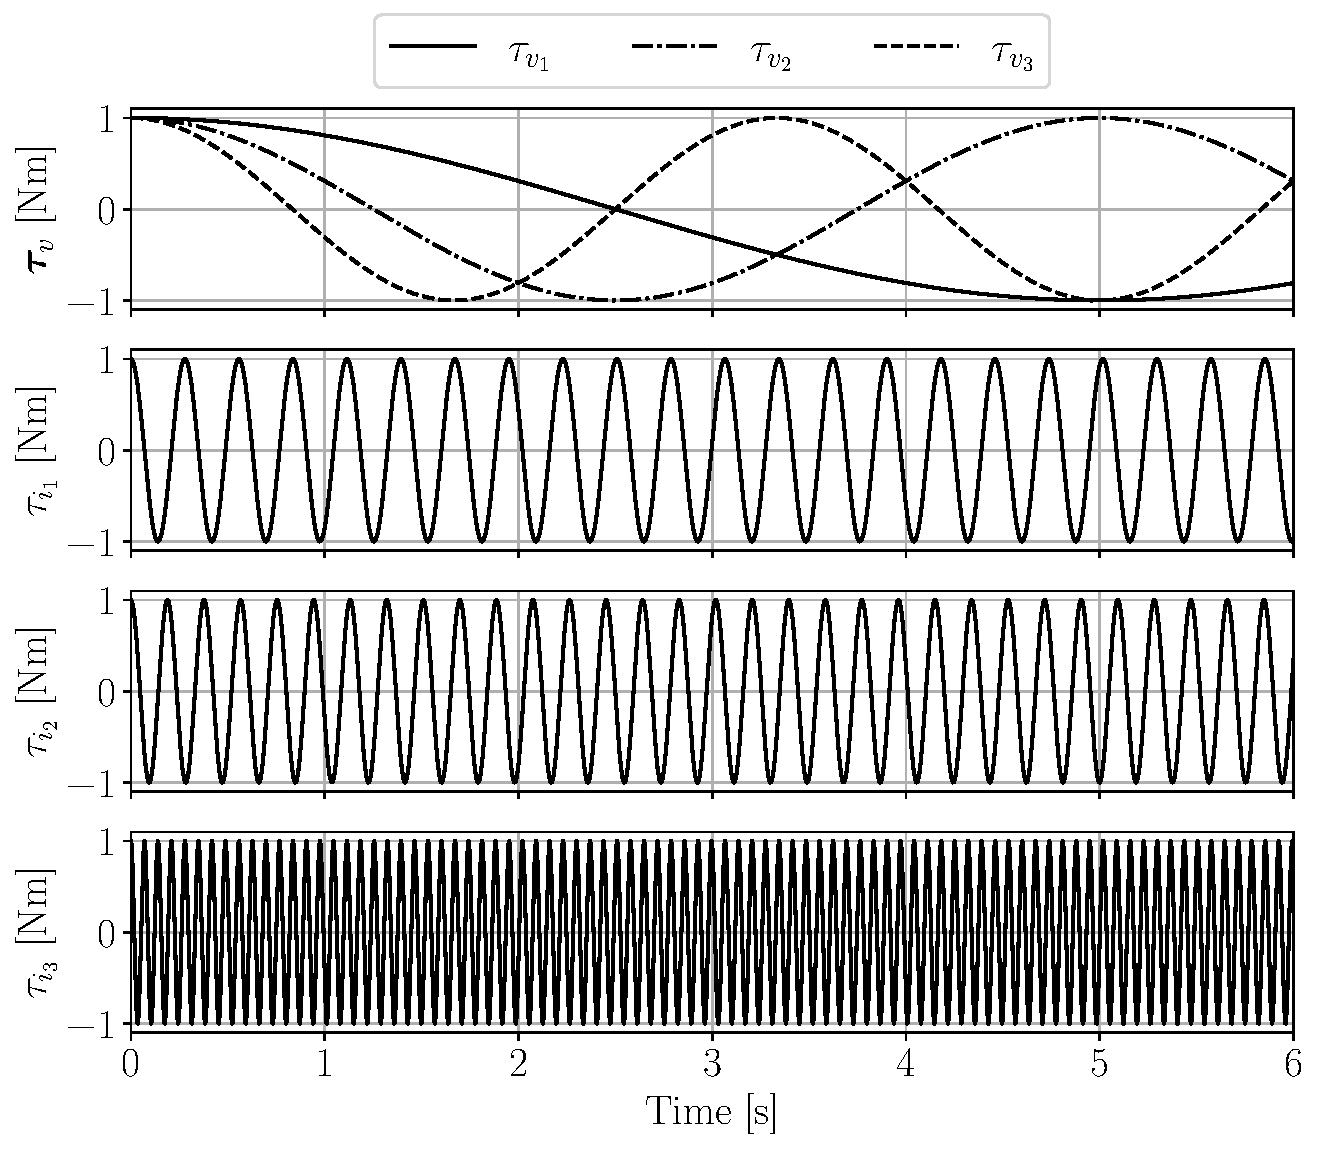
\includegraphics[width=\linewidth]{figures/plots/uncontrolled_amplitude_1.0/torque_profiles_uncontrolled_amplitude_1.0.pdf}
\end{figure}

Simulation results show that EADRC strategies effectively balance tremor attenuation and control effort in a coupled dynamic environment. 
While the DE-PID controller achieved a near-perfect TPSR above 99\%, it serves mainly as an ideal benchmark, relying on full knowledge of voluntary motion and requiring significantly higher actuation. Its TV was about 3.3 times that of EADRC with ZPLP in both scenarios.

\reviewchange{%
\begin{table*}[htbp]
    \centering
    \caption{
        Performance metrics of each control for $\bm\tau_v = \mathbf{0}$.
    }
    \label{tab:results_scenario1}
    \def\arraystretch{1.3}
    \begin{tabular}{
    c | c | c | c | c | c | c 
}
    \multirow{2}{*}{Controller} &
    \multicolumn{4}{c}{Response Signal} &
    \multicolumn{2}{|c}{Control Signal} \\
    \cline{2-7}
    &
    TPSR [\%] & 
    % ASR [\%] & 
    $R^2$ & 
    Entropy [bits] & 
    IAE [rad$\times$s] & 
    % ISE & 
    % ITAE & 
    % ITSE & 
    Power [(N$\times$m)$^2$] & 
    TV [N$\times$m$\times$s] 
    % IAC & 
    % ISC
\\
    \hline
%AFE & -150.62 $\pm$ 238.34 & -2.53 $\pm$ 1.94 & 5.36 $\pm$ 0.26 & 1.74 $\pm$ 0.45 & 0.76 $\pm$ 0.41 & 247.08 $\pm$ 71.96 \\
EADRC+EBMFLC & 40.67 $\pm$ 64.69 & 0.41 $\pm$ 0.14 & 5.19 $\pm$ 0.15 & 0.82 $\pm$ 0.26 & 0.49 $\pm$ 0.25 & 301.32 $\pm$ 83.25 \\
EADRC+ZPLP & 52.47 $\pm$ 46.16 & 0.44 $\pm$ 0.18 & 5.18 $\pm$ 0.17 & 0.73 $\pm$ 0.18 & 0.32 $\pm$ 0.12 & 255.43 $\pm$ 47.00 \\
%Gallego-PI & -147.98 $\pm$ 592.27 & -1.29 $\pm$ 2.18 & 5.08 $\pm$ 0.32 & 1.51 $\pm$ 1.10 & 2.21 $\pm$ 11.28 & 135.53 $\pm$ 46.99 \\
DE-PID & 99.90 $\pm$ 0.10 & 1.00 $\pm$ 0.00 & 4.85 $\pm$ 0.11 & 0.03 $\pm$ 0.01 & 0.88 $\pm$ 0.33 & 408.58 $\pm$ 8.93 \\
IMC-PID & -37.55 $\pm$ 279.40 & -0.16 $\pm$ 0.42 & 5.48 $\pm$ 0.14 & 1.13 $\pm$ 0.52 & 0.37 $\pm$ 0.23 & 183.32 $\pm$ 24.05 \\
\end{tabular}

\end{table*}
%
\begin{table*}[htbp]
    \centering
    \caption{
        Performance metrics of each control for $\bm\tau_v$ given by \eqref{eq:tau_v}.
    }
    \label{tab:results_scenario2}
    \def\arraystretch{1.3}
    \begin{tabular}{
    c | c | c | c | c | c | c 
}
    \multirow{2}{*}{Controller} &
    \multicolumn{4}{c}{Response Signal} &
    \multicolumn{2}{|c}{Control Signal} \\
    \cline{2-7}
    &
    TPSR [\%] & 
    % ASR [\%] & 
    $R^2$ & 
    Entropy [bits] & 
    IAE [rad$\times$s] & 
    % ISE & 
    % ITAE & 
    % ITSE & 
    Power [(N$\times$m)$^2$] & 
    TV [N$\times$m$\times$s] 
    % IAC & 
    % ISC
\\
    \hline
%AFE & -139.58 $\pm$ 315.12 & -1.63 $\pm$ 1.44 & 5.28 $\pm$ 0.25 & 1.72 $\pm$ 0.43 & 0.76 $\pm$ 0.35 & 229.81 $\pm$ 70.26 \\
EADRC+EBMFLC & 49.78 $\pm$ 51.24 & 0.46 $\pm$ 0.11 & 5.24 $\pm$ 0.13 & 0.82 $\pm$ 0.25 & 0.50 $\pm$ 0.24 & 301.84 $\pm$ 81.80 \\
EADRC+ZPLP & 61.31 $\pm$ 33.58 & 0.48 $\pm$ 0.16 & 5.24 $\pm$ 0.13 & 0.74 $\pm$ 0.18 & 0.33 $\pm$ 0.11 & 258.39 $\pm$ 43.92 \\
%Gallego-PI & -42.61 $\pm$ 132.60 & -0.66 $\pm$ 0.63 & 5.13 $\pm$ 0.24 & 1.38 $\pm$ 0.40 & 0.75 $\pm$ 1.15 & 124.11 $\pm$ 24.17 \\
DE-PID & 99.92 $\pm$ 0.08 & 1.00 $\pm$ 0.00 & 4.93 $\pm$ 0.10 & 0.03 $\pm$ 0.01 & 0.90 $\pm$ 0.34 & 409.52 $\pm$ 8.96 \\
IMC-PID & 4.79 $\pm$ 115.92 & -0.05 $\pm$ 0.33 & 5.48 $\pm$ 0.13 & 1.12 $\pm$ 0.45 & 0.40 $\pm$ 0.20 & 192.98 $\pm$ 20.43 \\
\end{tabular}

\end{table*}
}{%
    \begin{table*}[htbp]
        \centering
        \caption{
            Average performance metrics of each control strategy.
        }
        \label{tab:results_averages}
        \def\arraystretch{1.3}
        \begin{tabular}{
    c | c | c | c | c | c | c | c 
}
    &
    \multirow{2}{*}{Controller} &
    \multicolumn{4}{c}{Response Signal} &
    \multicolumn{2}{|c}{Control Signal} \\
    \cline{3-8}
    &&
    TPSR [\%] & 
    $R^2$ & 
    Entropy [bits] & 
    IAE [rad$\times$s] & 
    Power [(N$\times$m)$^2$] & 
    TV [N$\times$m$\times$s] 
\\
    \hline
    \multirow{4}{*}{\rotatebox{90}{$\bm{\tau}_v=\mathbf{0}$}}
    &
EADRC+EBMFLC & 40.67 $\pm$ 64.69 & 0.41 $\pm$ 0.14 & 5.19 $\pm$ 0.15 & 0.82 $\pm$ 0.26 & 0.49 $\pm$ 0.25 & 301.32 $\pm$ 83.25 \\ &
EADRC+ZPLP & 52.47 $\pm$ 46.16 & 0.44 $\pm$ 0.18 & 5.18 $\pm$ 0.17 & 0.73 $\pm$ 0.18 & 0.32 $\pm$ 0.12 & 255.43 $\pm$ 47.00 \\ &
DE-PID & 99.90 $\pm$ 0.10 & 1.00 $\pm$ 0.00 & 4.85 $\pm$ 0.11 & 0.03 $\pm$ 0.01 & 0.88 $\pm$ 0.33 & 408.58 $\pm$ 8.93 \\ &
IMC-PID & -37.55 $\pm$ 279.40 & -0.16 $\pm$ 0.42 & 5.48 $\pm$ 0.14 & 1.13 $\pm$ 0.52 & 0.37 $\pm$ 0.23 & 183.32 $\pm$ 24.05 
\\
    \hline
    \multirow{4}{*}{\rotatebox{90}{\tiny $\bm{\tau}_v$ as in \eqref{eq:tau_v}}}
    &
EADRC+EBMFLC & 49.78 $\pm$ 51.24 & 0.46 $\pm$ 0.11 & 5.24 $\pm$ 0.13 & 0.82 $\pm$ 0.25 & 0.50 $\pm$ 0.24 & 301.84 $\pm$ 81.80 \\ &
EADRC+ZPLP & 61.31 $\pm$ 33.58 & 0.48 $\pm$ 0.16 & 5.24 $\pm$ 0.13 & 0.74 $\pm$ 0.18 & 0.33 $\pm$ 0.11 & 258.39 $\pm$ 43.92 \\ &
%Gallego-PI & -42.61 $\pm$ 132.60 & -0.66 $\pm$ 0.63 & 5.13 $\pm$ 0.24 & 1.38 $\pm$ 0.40 & 0.75 $\pm$ 1.15 & 124.11 $\pm$ 24.17 \\
DE-PID & 99.92 $\pm$ 0.08 & 1.00 $\pm$ 0.00 & 4.93 $\pm$ 0.10 & 0.03 $\pm$ 0.01 & 0.90 $\pm$ 0.34 & 409.52 $\pm$ 8.96 \\ &
IMC-PID & 4.79 $\pm$ 115.92 & -0.05 $\pm$ 0.33 & 5.48 $\pm$ 0.13 & 1.12 $\pm$ 0.45 & 0.40 $\pm$ 0.20 & 192.98 $\pm$ 20.43 \\
\end{tabular}

    \end{table*}
}

\reviewchange{%
    In contrast, IMC-PID and Gallego-PI exhibited much lower TPSR, indicating sensitivity to coupled perturbations in a 3-DoF model.
}{% 
    To substantiate these comparisons statistically, a paired Wilcoxon signed-rank test was applied per metric and scenario, comparing EADRC+ZPLP against each baseline controller across the same 100 Monte Carlo parameter draws. 
    
    According to Table \ref{tab:wilcoxon}, in both scenarios EADRC+ZPLP outperforms EADRC+EBMFLC on every metric but Entropy ($p < 0.001$): 
    it achieves higher tremor suppression (TPSR, $r \geq 0.56$; IAE, $r \leq -0.68$) 
    while requiring less control effort (TV, $r \leq -0.81$), with lower control Power in every one of the 100 paired trials ($r = -1.00$), 
    supporting the claimed balance between attenuation and actuation. 
    Entropy did not differ significantly in the resting scenario ($p = 0.73$) and was moderately lower for EADRC+ZPLP in the moving one ($r = -0.32$). 
    
    Differences against DE-PID were significant for every metric in both scenarios with maximal or near-maximal effect size 
    ($|r| \geq 0.99$), reflecting that DE-PID suppressed tremor better than EADRC+ZPLP in practically every one of the 100 paired trials, 
    at the cost of higher control effort in all of them.
    %
    This is consistent with its role as an idealized upper-bound benchmark rather than a practical competitor.
    
    EADRC+ZPLP suppressed tremor better than IMC-PID in nearly every paired trial ($|r| \geq 0.94$ for TPSR, $R^2$ and IAE) 
    while requiring less control effort in every one of them (Power and TV, $r = -1.00$). 
    IMC-PID, tuned on the uncoupled nominal wrist, showed growing oscillations in 4 (resting) and 5 (moving) of the 99 perturbed models, 
    which explains its negative average TPSR despite median values above 50\%.
}

\reviewchange{}{
\begin{table}[htb]
    \centering
    \caption{% 
        Holm-Bonferroni corrected $p$-value and rank-biserial correlation $r$ 
        for paired Wilcoxon signed-rank tests.
    }
    \label{tab:wilcoxon}
    \resizebox{\linewidth}{!}{%
        \def\arraystretch{1.3}
        \begin{tabular}{c | c | cc | cc | cc}
    & \multirow{3}{*}{Metric} 
    & \multicolumn{6}{c}{EADRC+ZPLP vs. $\cdots$}
\\
\cline{3-8}
    &
    & \multicolumn{2}{c}{EADRC+EBMFLC} 
    & \multicolumn{2}{c}{DE-PID} 
    & \multicolumn{2}{c}{IMC-PID} \\
\cline{3-8}
    &
    & $p$ & $r$
    & $p$ & $r$
    & $p$ & $r$ \\
\hline
    \multirow{6}{*}{\rotatebox{90}{$\bm{\tau}_v = \mathbf{0}$}} & TPSR [\%] & 1.000 & -0.00 & $<$0.001 & -1.00 & $<$0.001 & +0.73 \\
    & $R^2$ & $<$0.001 & +0.53 & $<$0.001 & -1.00 & $<$0.001 & +0.97 \\
    & Entropy [bits] & $<$0.001 & -0.44 & $<$0.001 & +0.96 & $<$0.001 & -0.95 \\
    & IAE [rad$\times$s] & 1.000 & -0.03 & $<$0.001 & +1.00 & $<$0.001 & -0.81 \\
    & Power [(N$\times$m)$^2$] & 0.001 & -0.43 & $<$0.001 & -1.00 & 0.665 & -0.14 \\
    & TV [N$\times$m$\times$s] & 0.018 & -0.33 & $<$0.001 & -1.00 & $<$0.001 & +0.95 \\
\hline
    \multirow{6}{*}{\rotatebox{90}{$\bm{\tau}_v$ as in \eqref{eq:tau_v}}} & TPSR [\%] & 1.000 & +0.09 & $<$0.001 & -1.00 & $<$0.001 & +0.71 \\
    & $R^2$ & 0.039 & +0.31 & $<$0.001 & -1.00 & $<$0.001 & +0.99 \\
    & Entropy [bits] & 0.144 & -0.24 & $<$0.001 & +0.97 & $<$0.001 & -0.96 \\
    & IAE [rad$\times$s] & 1.000 & -0.08 & $<$0.001 & +1.00 & $<$0.001 & -0.76 \\
    & Power [(N$\times$m)$^2$] & $<$0.001 & -0.44 & $<$0.001 & -1.00 & 1.000 & -0.09 \\
    & TV [N$\times$m$\times$s] & 0.034 & -0.32 & $<$0.001 & -1.00 & $<$0.001 & +0.97 \\
\end{tabular}%
    }
\end{table}
}

While EADRC+ZPLP has been successful in suppressing tremor regardless of the voluntary motion estimator employed,
it demonstrated somewhat poor capacity in mitigating lower-frequency tremors, 
as spectrograms in Figure \ref{fig:plots} show.
%
This could indicate that the filtering process in voluntary motion estimation was not sufficient,
and EADRC did not factor unmitigated tremor as part of the total disturbance.

\begin{figure}[htb]
    \centering
    \captionof{figure}{Spectrograms of the uncompensated and compensated tremor of both scenarios.}
    \label{fig:plots}
    \begin{subfigure}{.685\linewidth}
        \centering
        \caption{Uncompensated resting tremor}
        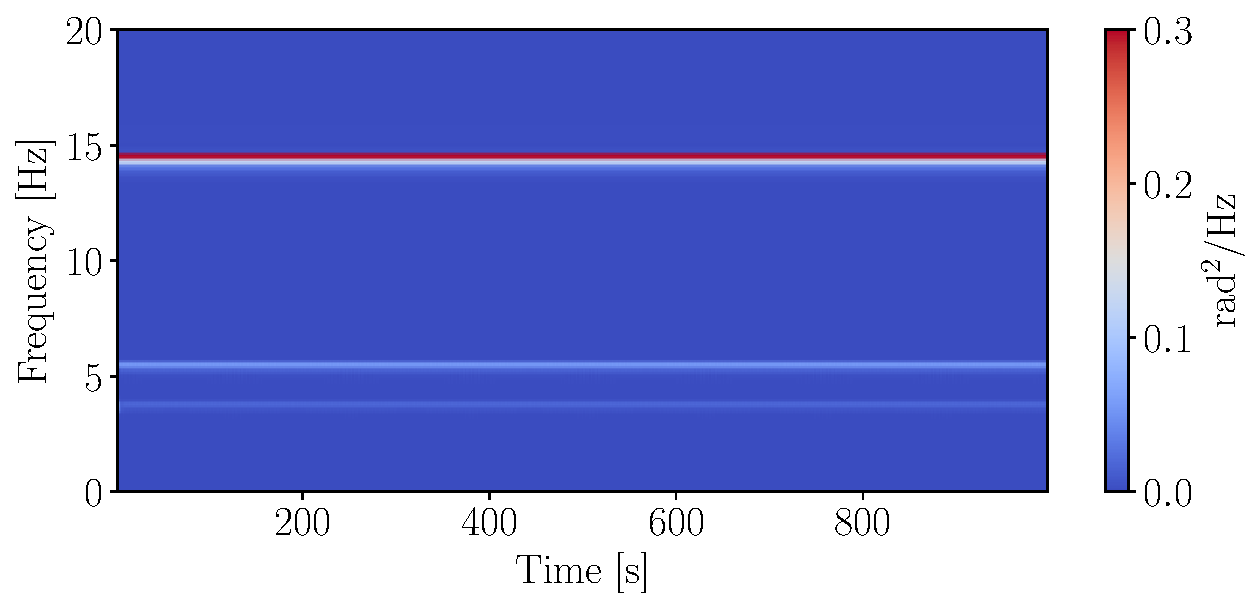
\includegraphics[width=\linewidth]{figures/plots/uncontrolled_amplitude_0.0/spectrogram_response_uncontrolled_amplitude_0.0.pdf}
    \end{subfigure}
    %
    \begin{subfigure}{.685\linewidth}
        \centering
        \caption{Compensated resting tremor}
        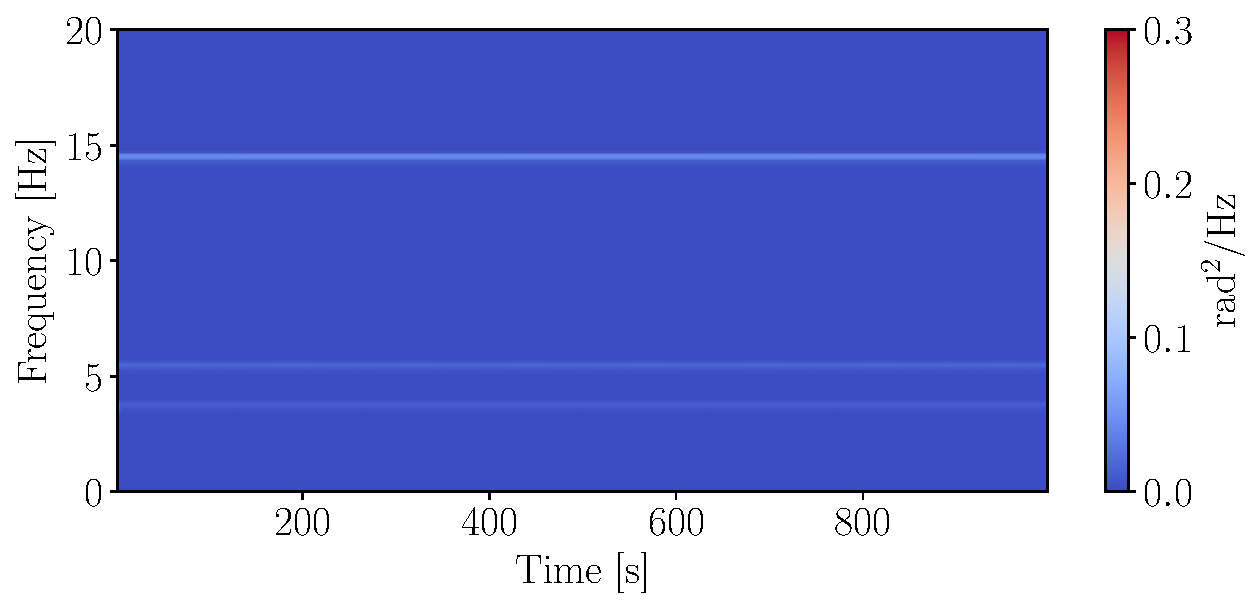
\includegraphics[width=\linewidth]{figures/plots/eadrc_ebmflc_amplitude_0.0/spectrogram_response_eadrc_ebmflc_amplitude_0.0.pdf}
    \end{subfigure}
    %
    \begin{subfigure}{.685\linewidth}
        \centering
        \caption{Uncompensated moving tremor}
        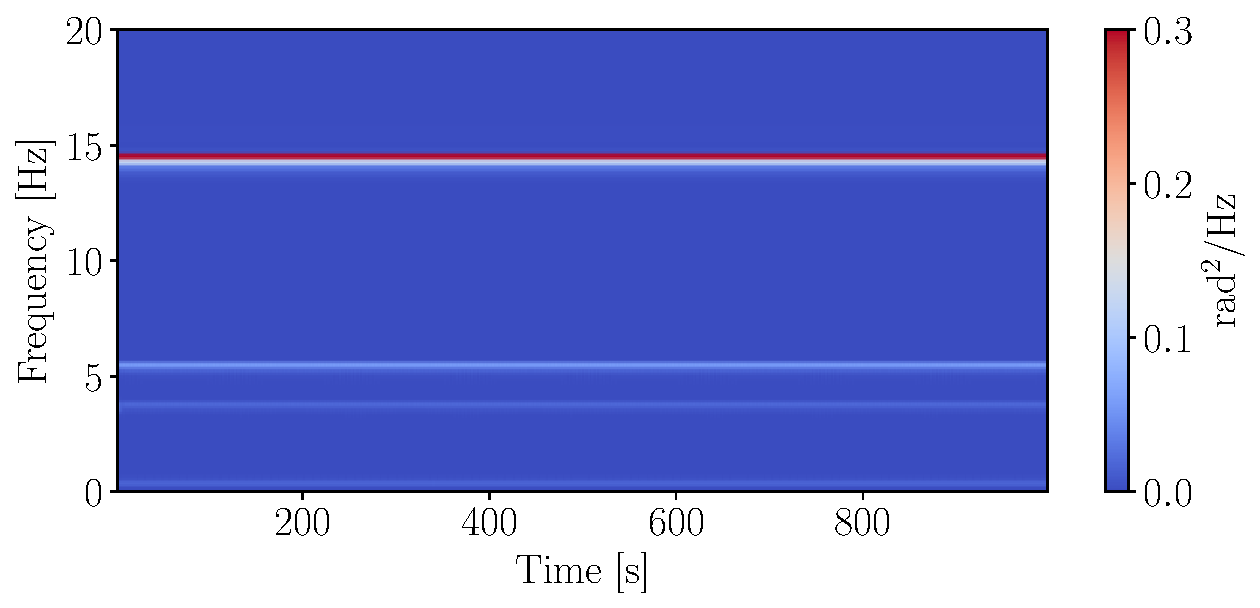
\includegraphics[width=\linewidth]{figures/plots/uncontrolled_amplitude_1.0/spectrogram_response_uncontrolled_amplitude_1.0.pdf}
    \end{subfigure}
    %
    \begin{subfigure}{.685\linewidth}
        \centering
        \caption{Compensated moving tremor}
        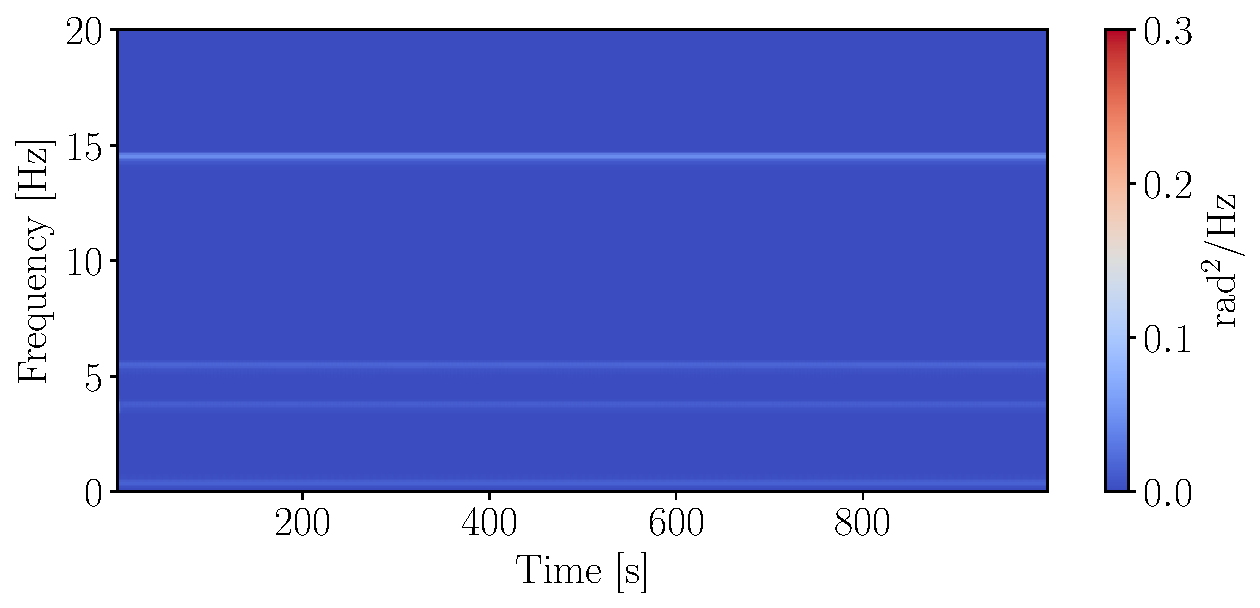
\includegraphics[width=\linewidth]{figures/plots/eadrc_ebmflc_amplitude_1.0/spectrogram_response_eadrc_ebmflc_amplitude_1.0.pdf}
    \end{subfigure}
\end{figure}
\section{Conclusion}
\label{sec:conclusion}

This work investigated error-based active disturbance rejection control for wrist tremor suppression in Parkinson's disease while accounting for upper limb dynamics. A 3-DoF mass-spring-damper model enabled the evaluation of control performance under disturbances arising from shoulder and elbow tremors. The results show that EADRC strategies, including EBMFLC and ZPLP variations, achieve high tremor power suppression with lower control effort than the more demanding DE-PID approach. 
%
\reviewchange{}{Of the two, EADRC+ZPLP achieved higher tremor suppression with smoother control signals.}
%
In particular, EADRC+ZPLP also reached an average tremor power suppression rate of 56.97\% in dynamic scenarios, outperforming classical controllers.

EADRC demonstrated strong robustness with both voluntary motion estimators used, maintaining consistent performance under variations of up to 50\% in joint stiffness and damping parameters. This indicates its suitability for practical applications where biomechanical properties are uncertain or time-varying. 
%
EADRC's ease of implementation and flexibility not withstanding, voluntary motion estimation is still key in avoiding the inclusion of lower-frequency tremors in the total estimated disturbance.
%
Future work will consider the inclusion of more control strategies from the literature, 
as well as the investigation of alternative voluntary motion estimation methods, and use of different upper limb models.

\bibliography{%
    references/active_disturbance_rejection_control_theory,%
    references/c1_tremor_characterization_reviews,%
    references/c2_tremor_suppression_reviews,%
    references/c3_passive_control_strategies,%
    references/c4_active_control_strategies,%
    references/metrics%
} 
\end{document}
